\section{Ziel}
In diesem Versuch sollen die Brechungs- und Beugungseigenschaften von Laserlicht betrachtet werden.
Dazu wird die Reflexion und Brechung in einem Plexiglasblock und die Beugung an mehreren Gittern betrachtet.

\section[Theorie]{Theorie\footnote[1]{Unter Verwendung von \cite{man:v400}.}}
% \subsection{Reflexion und Brechung}
\begin{wrapfigure}[12]{r}{5.5cm}
    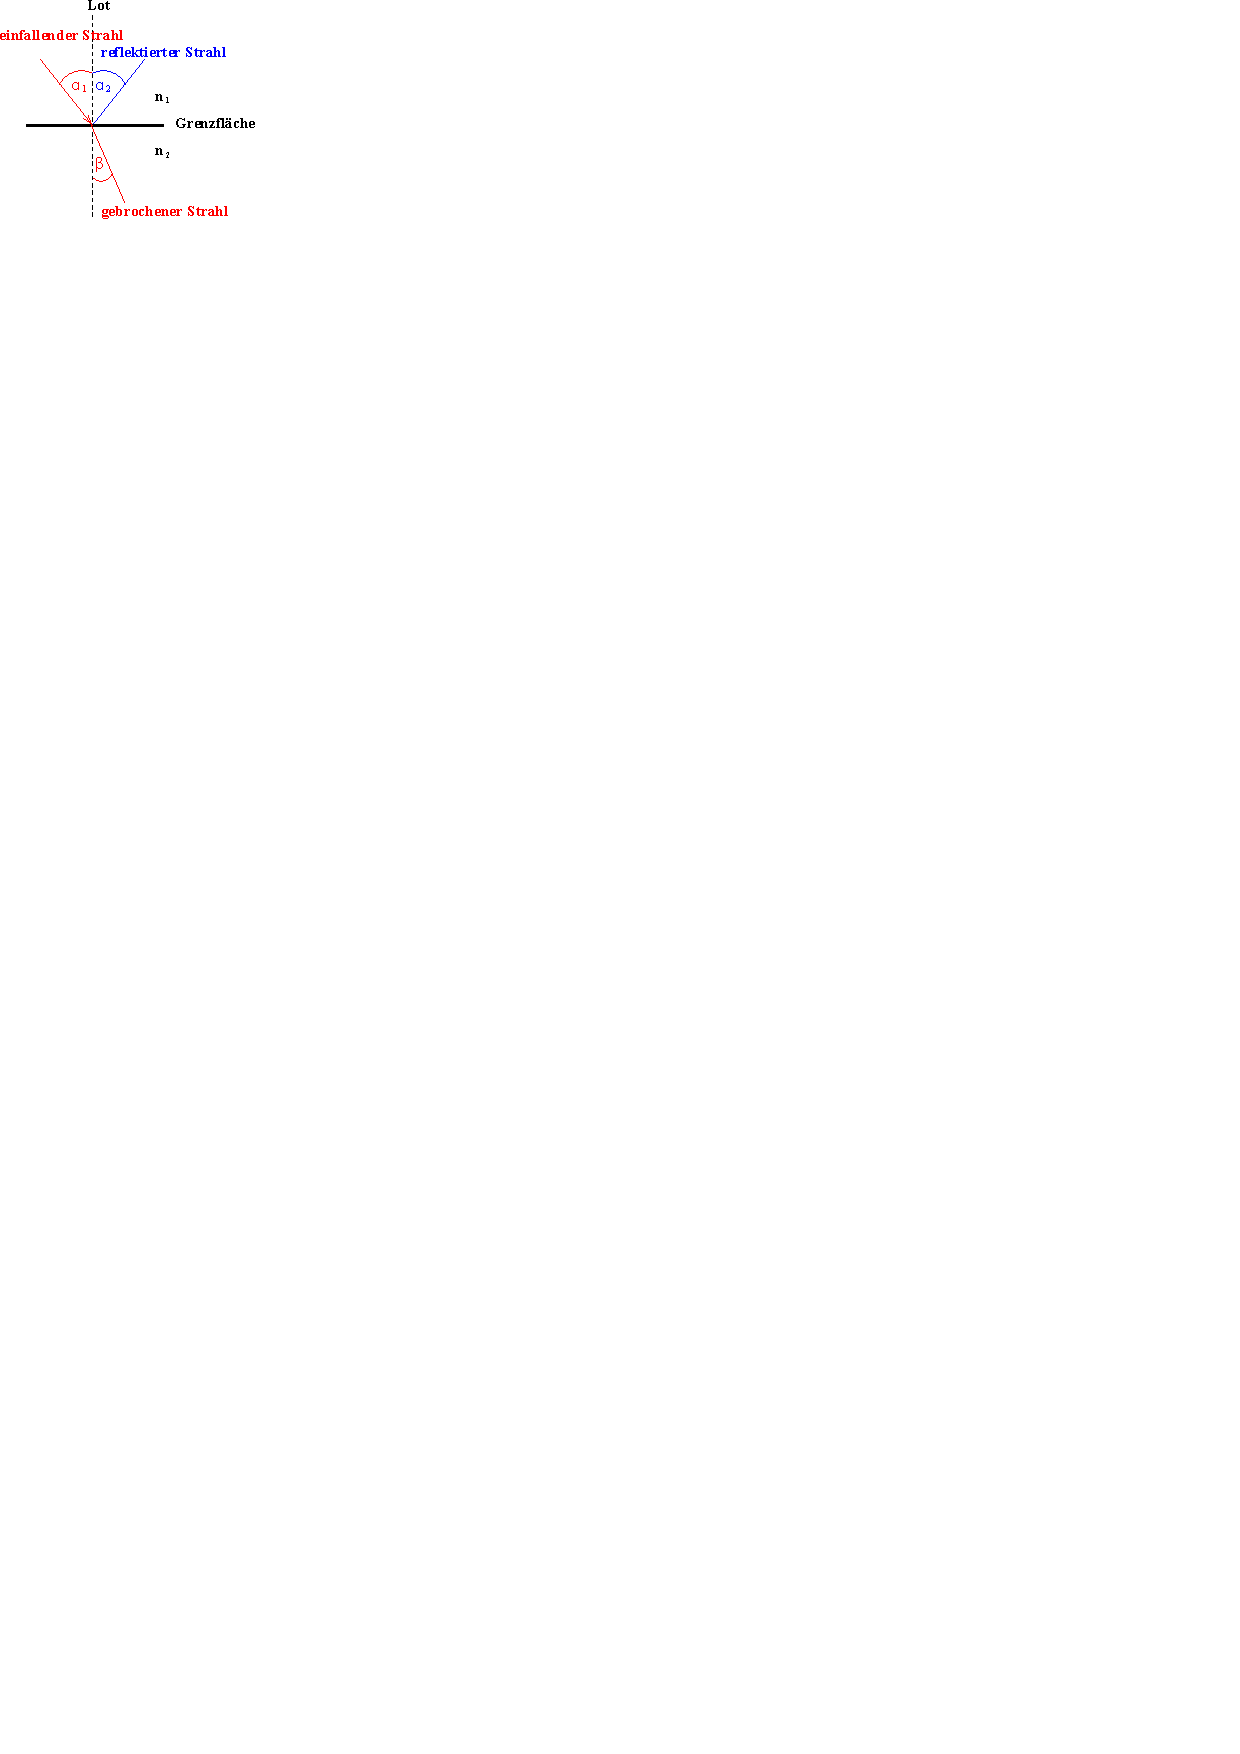
\includegraphics{Abbildungen/Ein_Ausfallwinkel.pdf}
    \caption{Ein- und Ausfallwinkel eines Lichtstrahls auf einer Grenzfläche \cite{man:v400}.}
    \label{fig:teo_refl_brech}
\end{wrapfigure}
Licht besteht aus elektromagnetischen Wellen.
Im Vakuum pflanzen sich alle EM-Wellen mit der gleichen Geschwindigkeit $c$ fort.
Im Medium ist diese Geschwindigkeit um 
\begin{align}
c'=c/n 
\label{eq:c_n}
\end{align}
verlangsamt.
Die veränderte Lichtgeschwindigkeit führt an glatten Oberflächen zu Brechungs- und Reflexionsphänomenen.
Die Strahlenoptik betrachtet EM-Wellen als gerade Strahlen, die geometrischen Gesetzen folgen.
Besonders relevant sind hier das Brechungsgesetz und das Reflexionsgesetz.
Nach dem Reflexionsgesetz ist der Einfallswinkel zur Flächennormalen gleich dem Ausfallswinkel des reflektierten Lichts.
\begin{align}
    \alpha_1 =\alpha_2
    \label{eq:reflexion}
\end{align}
Für das Brechungsgesetz werden die Winkel in dem anderen Medium in die das Licht eintritt mit $\beta$ bezeichnet.
Es gilt 
\begin{align}
    n_1 \sin(\alpha) = n_2 \sin(\beta).
    \label{eq:brechung}
\end{align}
Für Wellen die mit Objekten Interagieren, die eine vergleichbare Größe zur Wellenlänge haben 
treten zusätzlich noch Beugungseffekte auf.
Um diese korrekt zu beschreiben wird die Wellenoptik herangezogen.
Bei der Wellenoptilk ird das Licht als Wellenphänomen beschrieben.
Wellen können sich überlagern und sich gegenseitig verstärken sowie auch sich gegenseitig auslöschen.
In diesem Versuch wird die Beugung an einem Gitter betrachtet.
Das entstehende Beugungsmuster lässt sich mit dem Huygenschen Prinzip herleiten,
laut dem an dem Gitter viele kleine Elementarwellen entstehen und sich gegenseitig überlagern.
Für einen Schirm der durch ein Gitter mit einem Laser bestrahlt wird lässt sich ein Interferenzmuster herleiten.
Die k-ten Maxima auf dem Schirm liegen an folgenden Winkeln $\alpha$
\begin{align}
    d \sin{\alpha} = k \lambda.
    \label{eq:beugung}
\end{align}
$d$ ist hierbei der Gitterabstand.

Für den Versuch soll auch die Formel für den Strahlversatz $s$ bei zwei planparallelen Grenzflächen
\begin{align}
    s = d \frac{\sin(\alpha - \beta)}{\cos(\beta)}
    \label{eq:teo_strahlversatz}
\end{align}
bestätigt werden.
Eine Herleitung dieser Formel befindet sich in Abbildung \ref{fig:strahlversatz}.
\begin{figure}
    \centering
    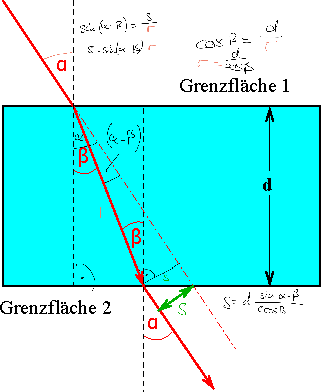
\includegraphics{Abbildungen/v400_strahlversatz.pdf}
    \caption{Herleitung von \eqref{eq:teo_strahlversatz} anhand der Abbildung aus \cite{man:v400}}
    \label{fig:strahlversatz}
\end{figure}

Für das Prisma in Abbildung \ref{fig:prisma} soll eine Gleichung für $\delta$ aufgestellt werden.
Sie lautet
\begin{align}
    \delta = (\alpha_1 + \alpha_2) - (\beta_1 + \beta_2). %% Achtung diese Gleichung ergibt hier nicht unbedingt Sinn!
    \label{eq:prisma}
\end{align}

\begin{figure}
    \centering
    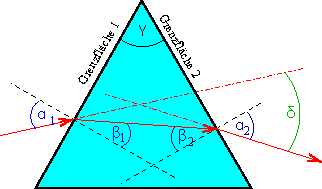
\includegraphics{11_v400/Abbildungen/Prisma.pdf}
    \caption{Ein- und Ausfallwinkel an einem Prisma}
    \label{fig:prisma}
\end{figure}

\subsection{Vorbereitungsaufgaben Strahlversatz und Prisma}

\begin{table}
    \centering
    \begin{tabular}{c S }
        \toprule
        Material & {Brechungsindex}\\
        \midrule
        Luft        & 1.00029   \\
        Wasser      & 1.333     \\
        Kronglas    & 1.51      \\
        Plexiglas   & 1.49      \\
        Diamant     & 2.42      \\           
    \end{tabular}
    \caption{Brechungsindizes verschiedener Materialien \cite{brechungsindex}.}
    \label{tab:brechungsindex}
\end{table}

\begin{table}
    \centering
    \begin{tabular}{S S}
        \toprule
        {$N  /(\unit{1 \per \mm}) $} & {$d / \unit{\micro\m}$} \\
        \midrule
        600 &  1.67 \\ 
        300 &  3.33 \\ 
        100 &  10  \\
        \bottomrule
    \end{tabular}
    \caption{Gitterkonstanten $d$ bei verschieden Gittern mit $N$ Linien/\unit{\mm}}
    \label{tab:gitterkonstanten}
\end{table}

In den Tabellen \ref{tab:brechungsindex} und \ref{tab:gitterkonstanten} sind die Brechungsindizes verschiedenener
Materialien und die Gitterkonstanten verschiedener Gitter angegeben. 

